\section{Requirement Analysis and Specifications Document}

The Requirements and Specifications Document (RASD) serves several purposes:
\begin{itemize}
    \item Communication: it conveys an understanding of the requirements, encompassing the application domain and the system under development.
    \item Contractual: it can be legally binding, serving as a formal agreement between stakeholders.
    \item Baseline for project planning and estimation: it provides a foundation for project planning and estimation, covering aspects like size, cost, and schedule.
    \item Baseline for software evaluation: it supports system testing, verification, and validation activities. 
        It contains the information necessary to verify if the delivered system aligns with the requirements.
    \item Baseline for change control: it establishes a foundation for managing changes in requirements as the software evolves.
\end{itemize}
The RASD document is utilized by various stakeholders, including:
\begin{itemize}
    \item Customers and Users: they are interested in a high-level description of system functionalities and requirements.
    \item System analyst and requirement analysts: these individuals use the RASD to specify how the system interacts with other systems.
    \item Developers and programmers: they refer to the RASD for implementation details.
    \item Testers: they use the RASD to check if the system meets its requirements.
    \item Project managers: they rely on the RASD to control the development process.
\end{itemize}
\begin{figure}[H]
    \centering
    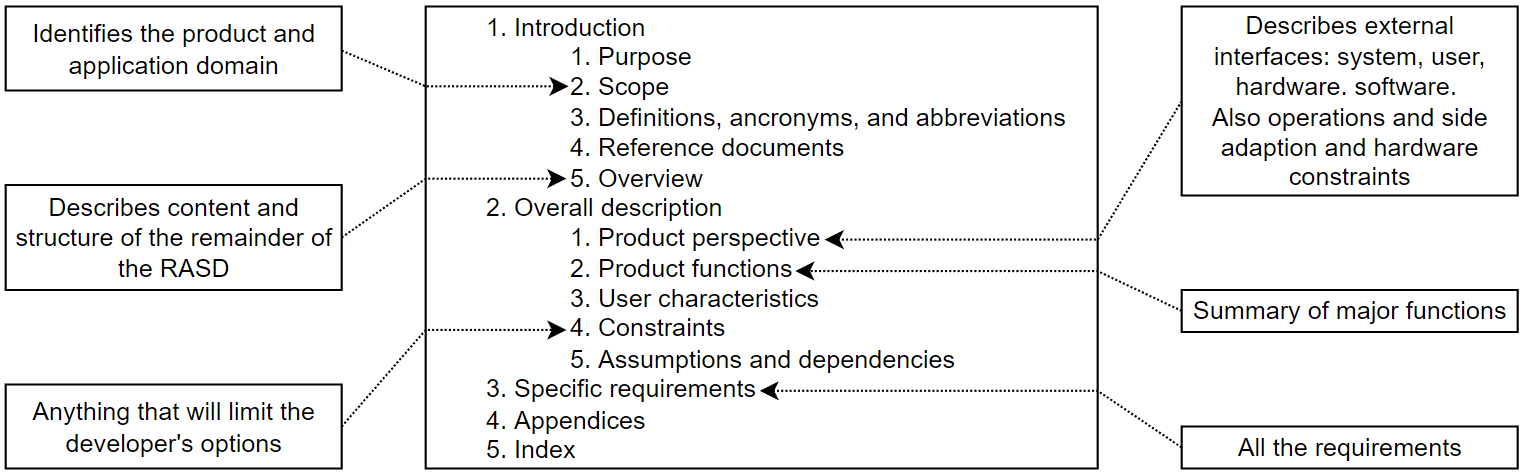
\includegraphics[width=0.5\linewidth]{images/RASD.png}
    \caption{IEEE standard for RASD}
\end{figure}